\documentclass[14pt,a4paper]{article}

% =================== PACOTES ===================
\usepackage[utf8]{inputenc}
\usepackage[T1]{fontenc}
\usepackage[brazil]{babel}
\usepackage{graphicx}   % para inserir o logo
\usepackage{setspace}   % espaçamento
\usepackage{geometry}   % margens
\usepackage{tcolorbox}  % caixas de solução
\usepackage{fancyhdr}   % cabeçalho e rodapé
\usepackage{float}
\usepackage{caption}
\tcbuselibrary{theorems}
\usepackage{listings}   % Para exibir código fonte
\usepackage{xcolor}

\geometry{a4paper, top=3cm, bottom=2.5cm, left=3cm, right=2.5cm}

% =================== CABEÇALHO ===================
\pagestyle{fancy}
\fancyhf{}
\fancyhead[L]{Maykon Hopka -- 23203081}  
\fancyfoot[C]{\thepage}

% =================== AMBIENTE DE SOLUÇÃO ===================
\newtcbtheorem[number within=section]{solucao}{Solução}%
{colback=green!5,colframe=green!60!black,fonttitle=\bfseries}{sol}

% =================== CAPA ===================
\begin{document}
\begin{titlepage}
    \centering
    
    
\includegraphics[width=0.25\textwidth]{logo_ufsc.png}\par\vspace{1cm}
    
    {\Large\bfseries Universidade Federal de Santa Catarina \par}
    \vspace{0.5cm}
    {\large Centro de Engenharias da Mobilidade \par}
    {\large Curso de Engenharia Mecatrônica \par}
    \vfill
    
    {\Huge\bfseries Impasses \par}
    \vspace{0.5cm}
    {\Large Disciplina: Sistemas Operacionais\par}
    \vspace{0.3cm}
    {\large Aluno: Maykon Hopka \par}
    \vfill
    
    {\large Joinville – 2025}
\end{titlepage}

% =================== CONTEÚDO ===================
\section{Exercícios}

\subsection*{Exercício 1}
A alteração em qual fator aumentou a quantidade de travamentos no programa

\begin{solucao}{Exercício 1}{}
 Aumentar o numero de threads e transferências
\end{solucao}

\subsection*{Exercício 2}
Faça a modelagem do grafo de alocação de recursos para explicar a razão do programa travar

\begin{solucao}{Exercício 2}{}
\begin{figure}[H]
    \centering
    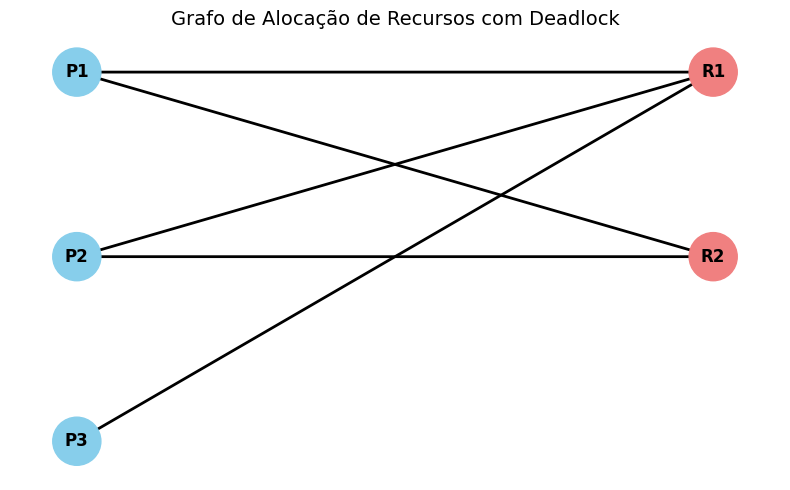
\includegraphics[width=0.5\textwidth]{grafo.png}
    \caption{Grafo de alocação de recursos mostrando deadlock}
    \label{fig:grafo}
\end{figure}

\begin{itemize}
    \item No sistema, temos três processos (P1, P2 e P3) e dois recursos compartilhados (R1 e R2).
    \item O processo \textbf{P1} está de posse do recurso \textbf{R1} e solicita \textbf{R2}.
    \item O processo \textbf{P2} está de posse do recurso \textbf{R2} e solicita \textbf{R1}.
    \item O processo \textbf{P3} solicita \textbf{R1}, mas não consegue obtê-lo, pois ele está alocado para P1.
    \item Neste cenário, há um ciclo de espera entre P1 e P2:
    \begin{itemize}
        \item P1 → R2 (espera por R2, que está com P2)
        \item P2 → R1 (espera por R1, que está com P1)
    \end{itemize}
    \item Esse ciclo caracteriza um \textbf{deadlock}, pois os processos ficam esperando indefinidamente pela liberação de recursos uns dos outros.
    \item O processo P3 está bloqueado, mas não causa o deadlock diretamente — ele apenas aguarda a liberação de um recurso envolvido no ciclo.
\end{itemize}

\textbf{Resumo:} O programa pode travar quando múltiplas threads tentam adquirir os mesmos semáforos em ordens diferentes. Se a thread A segura o semáforo da conta 1 e tenta acessar a conta 2, enquanto a thread B segura o semáforo da conta 2 e tenta acessar a conta 1, nenhuma das duas prossegue — esse é o cenário modelado pelo grafo de alocação de recursos com deadlock.

\end{solucao}


\subsection*{Exercício 3}
Pergunte à sua IA favorita (GPT, Gemini, etc) para encontrar uma solução e teste se a solução proposta realmente funciona.

\begin{solucao}{Exercício 3}{}
Para evitar esse problema, a IA sugeriu u: \textbf{sempre adquirir os semáforos na mesma ordem}, independentemente de qual conta é origem ou destino. A ordem foi definida com base no número da conta (ID). Assim, elimina-se a possibilidade de deadlock.

\begin{verbatim}
// Transferência com ordenação de semáforos para evitar deadlock
void transferir (conta_t *contaDeb, conta_t *contaCred, float valor){
    conta_t *primeira, *segunda;

    // Ordena os locks para sempre adquirir na mesma ordem
    if (contaDeb->numero < contaCred->numero) {
        primeira = contaDeb;
        segunda = contaCred;
    } else {
        primeira = contaCred;
        segunda = contaDeb;
    }

    sem_wait(&(primeira->trava));
    sem_wait(&(segunda->trava));

    if(contaDeb->saldo >= valor){
        contaDeb->saldo -= valor;
        contaCred->saldo += valor;
    }

    sem_post(&(segunda->trava));
    sem_post(&(primeira->trava));
}

// Correção na função da thread
void *auxThread(void *arg){
    int origem,destino;
    long n_trans=(long)arg;
    float valor;
    for (int i=0;i<n_trans;i++){
        origem = random() % n_contas;
        destino = random() % n_contas;
        while(destino == origem){
            destino = random() % n_contas;
        }
        valor = 1.0 * (random() % 10);
        transferir(&contas[origem], &contas[destino], valor);
    }
    pthread_exit(NULL); // Encerra a thread corretamente
}
\end{verbatim}

\textbf{Resultado:} Com essas modificações, o programa do Gepeto(ChatGPT) pareceu funcionar nos meus testes.
\end{solucao}
% =================== FIM ===================

\end{document}
